\documentclass[conference]{IEEEtran}
\IEEEoverridecommandlockouts
% The preceding line is only needed to identify funding in the first footnote. If that is unneeded, please comment it out.
\usepackage{cite}
\usepackage{amsmath,amssymb,amsfonts}
\usepackage{algorithmic}
\usepackage{graphicx}
\usepackage{textcomp}
\usepackage{xcolor}
\usepackage[german]{babel}

\def\BibTeX{{\rm B\kern-.05em{\sc i\kern-.025em b}\kern-.08em
T\kern-.1667em\lower.7ex\hbox{E}\kern-.125emX}}
\begin{document}

\bibliographystyle{IEEEtran}
\graphicspath{imgs}

\title{Erkennung von Design Patterns durch Maschine Learning}

\author{\IEEEauthorblockN{1\textsuperscript{st} Mehmet Aslan}
    \IEEEauthorblockA{\textit{Fakultät für Informatik} \\
        \textit{Hochschule Rosenheim}\\
        Rosenheim, Deutschland \\
        mehmet.aslan@stud.th-rosenheim.de}}

\maketitle
\thispagestyle{plain}
\pagestyle{plain}

\begin{abstract}
    Diese Seminararbeit setzt sich den Fokus, wie mithilfe von Machine Learning das Problem der Erkennung von Design Patterns erläutert. Dabei wird definiert, was unter Design Patterns im Rahmen dieser Seminararbeit zu verstehen und welchen Mehrwert die automatisierte Erkennung von diesen mit sich bringt.
    Zudem werden Ansätze erläutert, die diese Problematik ohne Einsatz von Machine Learning lösen. Als finaler Abschnitt werden die groben notwendigen Schritte vorgestellt, wie die Erkennung von Design Patterns durch maschinelles Lernen gelöst werden kann. Dabei werden Prozesse vorgestellt, die sich mit dieser Thematik befassen und wie diese den entsprechenden Schritt umgesetzt haben.
\end{abstract}

\begin{IEEEkeywords}
    Machine Learning, Design Pattern Detection
\end{IEEEkeywords}

\section{Einleitung}
In der Entwicklung von Software-Systemen werden im Öfteren auf Probleme gestoßen, die bereits in der gleichen oder in ähnlicher Form bereits gelöst wurden. Für diese gängigen Probleme haben sich im Gegenzug gängige Lösungsblaupausen etabliert, womit sich diese lösen lassen.
Dadurch, dass Software-Systeme durch neue oder angepasster Änderungen sich inkrementell weiterentwickeln, ist die strukturelle Verbesserung und Neugestaltung des unterliegenden Quellcodes ohne Veränderung des Programmverhaltens, auch Code-Refactoring genannt, Teil des Entwicklungsprozesses.
Bei komplexen Software-Systemen werden auch Design Patterns verwendet. Bei Code-Refactoring muss man den gewissen Systemkontext während des Prozesses im Kopf beibehalten, um den betrachte Programmfluss im Quellcode zu verstehen.
Dabei können Programmstrukturen über mehreren Quellcode-Dateien, Module oder Bibliotheken verteilt sein. Deshalb kann der Erhalt des Systemkontextes im Verständnis schwerfallen, vor allem bei Design Patterns. Um dagegenzuwirken, kann werkzeug-gestützte Hilfestellung mithilfe von Machine Learning den Refactoring-Prozess mit Umgang von Design Patterns einfacher gestalten.
Diese Seminararbeit setzt sich die Untersuchung der Erkennung von Design Patterns mit Machine Learning als Fokus. Dabei ist die Arbeit in folgende Segmente untergliedert: gesetzte Einschränkung für die Untersuchung, Ansätze aus nicht Machine Learning Gebieten und die notwendigen Schritte für die Erstellung eines Modells durch Vergleich verschiedener bereits untersuchter Prozesse.

%TODO: Add findinngs here


\section{Eingrenzungen der Seminararbeit}
Um mit der Erkennung der Design Patterns anzufangen, muss vorerst definiert werden, welche Design Patterns überhaupt zu betrachten sind. Da der Fokus dieser Seminararbeit auf der Analyse von Quellcode liegt, werden hier deren Einsatz in Programmiersprachen betrachtet.
Das Werk, was den Begriff der Design Patterns in den Köpfen den Software-Entwicklern am ehesten assoziieren, sind die Konstrukte, die im Werk "Design Patterns: Elements of Reuseable Software" definiert. Diese Design Patterns sind ebenfalls unter dem Begriff ``GoF Design Patterns'' bekannt. Da der Fokus in diesem Werk den Einsatz von Design Patterns in einem
objektorientierten Kontext betrachtet werden, wird diese auch so im weiteren Verlauf der Untersuchung übernommen. Obwohl die Erläuterungen der GoF Design Patterns ursprünglich in der Programmiersprache C++ verfasst wurden, wird in dieser Arbeit deren Einsatz ebenfalls in anderen objektorientierten Programmiersprachen betrachtet.
Dabei werden die Design Pattern in folgende Kategorien unterteilt werden \cite[p. 5797]{Yarahmadi2020}:

\begin{figure}[h]
    \centering
    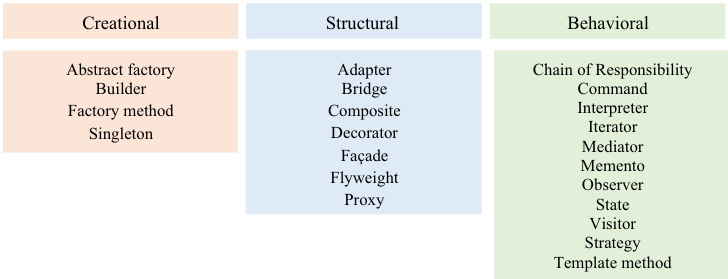
\includegraphics[width=\linewidth]{imgs/gof.png}
    \caption{Design Pattern Kategorien nach GoF}
\end{figure}


\newpage

\section{Alternative Ansätze}

Neben den Lösungsansätzen aus dem Machine Learning Bereich, wurden Verfahren aus anderen Bereichen der Informatik eingesetzt, um die Erkennung von Design Patterns bis zu einem gewissen Grad zu automatiesiern.
In diesem Abschnitt der Seminararbeit werden einige Ansätze vorgestellt.

\subsection{Graphenanalyse}

In den meisten Verfahren ist der Quellcode in seiner ursprünglichen Form als Textdatei als Input nicht geeignet, um mit einer hohen Genauigkeit Design Patterns zu erkennen.
Aus diesem Grund ist daher notwendig, dass man die Quelldateien in eine andere Form transformiert, um mit diesen besser arbeiten zu können. Deshalb ist die Transformation der Quelldateien in eine graphenbasierte Form ein bereites etablierter Ansatz.
Durch den Einsatz von Knoten, Kanten und Subgrapehn können die Beziehung und Zusammensetzung der einzelnen Komponenten in den Quelldateien in einer proagrammiersprachenagnostischen Form repräsantiert werden.
Dabei dienen Eigenschaften von Graphen und graphenbasierte Algorithmen wichitige Werkzeuge in diesen Ansätzen. Besipielsweise wird in der Arbeit von Pradhan et al. \cite{PradGraph} die Eigenschaften der Graphenisomorphie, um aus dem Quellecode-Graphen, Design Patterns zu erkennen.
Dabei ist das zu suchende Desgin Pattern als Subgraph Teil des Quellcode-Graphen. Darin wird mithilfe eines bereits definierten Graphen, was ein Design Pattern dartsellt, nach isomorphen Teilgraphen im Quellcode-Graphen gesucht.
Zusätzlich wird die normalisierte Kreuzkorrelation genutzt, um die Ähnlichkeit zwischen den gefundenden Teilgraphen und dem gesuchten Desgin Pattern zu qunatifizieren.
Ein weiteres Bespiel wäre der Ansatz von Bernardi et al., die eine domänspezifische Sprache entwickelt, womit Desgin Patterns als ein Set von Regeln definiert werden kann \cite{Bernardi2013AMG}. Diese Regeln werden dann genutzt, um Muster im Quellcode Graphen zu erkennen.

\subsection{Analyse durch Software-Metriken}

Um gestützte Aussagen über Software-System zu tätigen, werden in der Software-Entwicklung Metriken eingesetzt, um Eigenschaften wie Größe, Komplexität, Kopplug usw. des betrachteten Software-Systems zu qunatifizieren.
Dadruch erschließt sich die Möglichkeit, Hypothesen über das Software-System zu tätigen. Diese Metriken können bei der Erkennung von Design Patterns genutzt werden als indirekter Anstz genutzt werden, um Anzeichen oder Muster in einem Software-System zu erkennen.
In ihrer Arbeit schlagen Issaoui et al. \cite{Issaoui2015} einen Prozess vor, wie mithilfe von Software-Metriken der Suchraum für Design Patterns eingeschränkt werden kann. Dabei werden konkrete Eigenschaften und Metrikwerte bestimmt, die das jeweilige Design Pattern.
Das gesamte zu betrachtende Software-System wird durch die vorher definierten Metriken quantifiziert und es werden diejenigen Komponenten des Software-Systems weiterbetrachtet, die die vorher festgelegten Konstrikte erfüllen.
Dieser Ansatz dient als ergänzende Methodik für existierende Prozesse, um die Menge möglicher Kanidaten zu reduzieren.
Ashish et al. hingegen nutzen Software-Metriken, um ein Dataset zu generieren, die Design Patterns verschiedene Software-Metriken und Werte zu ordnen \cite{Ashish2016}. Dabei dient dieses Dataset als Eingabe für Data Mining- und maschinelle Lernalalgorithmen, um Relationen zwischen Software-Metriken und Design Patterns abzuleiten.


\subsection{Analyse durch Anfragen}

Dieser Ansatz orinetiert sich an relationalle Datenbanken. Dabei wird an ein Set von Daten eine Anfrage gestellt und als Ergebnis wird ein Subset der Daten zurückgegeben, die die Bedingungen der gestellten Anfrage erfüllen.
Daher muss das Software-System in eine Form transformiert, an diesem die Anfragen durchgeführt werden können. Dazu eignenen sich baumartige Formate wie Abstract Syntax Trees (AST) oder Extended Markup Language Dokumente.
ASTs werden bei dem Compile-Vorgang verwendet, um die Struktur des jeweiligen Quellcodes zu repräsentieren. XML-Dokumente erfüllem einen ähnlichen Zweck wie AST in diesem Kontext,
bieten zusätzlich die Möglichkeit an, durch Einsatz von Attributen zusätzliche Meta-Informationen mitzugeben. Diese Strukturen ermöglichen das Traversieren der jeweiligen Struktur durch Angabe von der zu begehenden Pfade in Form von Anfragen.
Die gesuchten Design Patterns werden in Form dieser Anfragen abgelegt und durch an der jeweiligen Baumstruktur durchgeführt.
Bouassida und Ben-Abdallah stellen einen Prozess wie mithilfe von Information-Retrieval-Techniken, Artefakte des Quellcodes wie Klassen, Methoden oder Beziehungen zwischen Entitäten als XML-Dokument zu repräsentieren \cite{bouassida2010pattern}.
Mit Anfragen können nun in diesem Ansatz durch Anfragen nach Design Patterns oder nach "spoiled patterns", abgewandelten Design Patterns, gesucht werden.

%TODO: \subsection{Analys durch FC} Falls notwendig

\newpage

\section{Machine Learning Ansatz: Grober Ablauf}

Das Erscheinen von kostenlosen Open-Source Projekten wie TensorFlow, sklearn oder PyTorch sorgte dafür, dass im Verlauf der Jahre der Zugang und die Einstiegshürde geringer wurde, sodass der Einsatz von Machine Learning
weiter zunahm. Machine Learning Algorithmen sind unteranderem dafür geeignet, um Eingaben zu klasszifieren, neue synthetische Daten zu generieren oder eine Regressionsanalyse durchzuführen. Im Feld der Design Pattern Erkennung wurde Machine Learning basierende Anätze als Kern bei dem Erkennungsprozess oder wurden als ergänzender Schritt in den Prozess hineingearbeitet und fand dadurch immer weiter Ansatz \cite[p. 5805]{Yarahmadi2020}.
In diesem Abschnitt der Seminararbeit werden grob die notwendigen Schritte vorgestellt, wie theoretisch solch ein Prozess mit Machine Learning im Kern aussehen kann.

\subsection{Data Gathering}
In dem initialen Zustand ist ein untraniertes Machine Learning Modell blank. In dieser Situation ist Modell nicht in der Lage, die erwarteten Anforderungen zu erfüllen, da das Modell kein Wissen über die Eingaben besitzt. Aus diesem Grund muss notwendige Wissen dem Modell beigebracht werden.
Data Gathering beschreibt im Machine Learning Prozess, wie die Rohdaten zu einem Kollektiv zusammengetragen, die im weiteren Verlauf der Seminararbeit als Dateset betrachtet wird. Dabei sollte beachtet werden, dass es sich hierbei um Rohdaten handelt. Die Daten werden in deren darauf folgenden Schritten weiter bearbeitet.
Für die Erstellung des Datasets eignen im Kontext der Design Pattern Erkennung für Machine Learning vorallem Open-Source Projekte. Viele der Prozesse nutzen Quelldateien als unverarbeite Eingabe \cite[p. 5801]{Yarahmadi2020}, die in den darauffolgenden Phasen um Informationen ergänzt oder transformiert werden. Open-Source eignen sich hierfür, da Lizens meistens das freie Weiternutzen der Quelldateien ermöglichen.
Folgende Open-Source werden am meisten verwendet \cite[p. 5817]{Yarahmadi2020}:

\begin{itemize}
    \item JUnit
    \item JHotDraw
    \item JRefactory
    \item Java AWT
\end{itemize}

\subsection{Explorativ Data Analysis}

Explorativ Data Analysis (EDA) beschäftigt sich mit der Analyse des Datasets, um Muster, Trends, Abweichungen oder andere relevante Informationen im Dataset zu identifizieren.
Das Hauptziel von EDA besteht darin, ein besseres und tieferes Verständnis für das Dataset zu gewinnen, bevor das Dataset weiter verarbeitet wird. Dabei werden verschiedene Methoden und Techniken verwendet,
um die Daten zu visualisieren, Beziehungen zwischen Eingabenvariablen und statistische Analysen durchzuführen. Je nach Dataset bereits darauffolgende Schritte wie Data Cleaning oder Feature Extraction bereits hier durchgeführt werden.
Dabei können je nach Verfügbarkeit des Datasets folgende Methoden und Techniken hilfreich sein:

\begin{itemize}
    \item \textbf{Data Visualization}: Durch Einsatz von Diagrammen, Plots oder Histogrammen können Muster, Trends oder Ausreißer im Dataset erkannt werden
    \item \textbf{Statiscal Analysis}: Methoden wie Mittelwerte, Varianzen, Korrealtionen oder Clusteranalysen können statistische Zusammenhänge bereits im Vorfeld erkannt werden
\end{itemize}


\subsection{Data Preprocessing}

Data Preprocessing beschreibt den notwendigen Schritt, um die Rohdaten in eine Form zu bringen, mit denen das Machine Learning Modells umgehen kann.
Dieser Schritt beinhaltet unteranderem die Bereinigung, Transformation und Formatierung der Rohdaten. Dadurch kann die Leistungsfähigkeit des ausgewählten Modells verbessert werden.
Im Kontext der Design Pattern Erkennung können folgende Schritte von Bedeutung sein:

\begin{itemize}
    \item \textbf{Data Cleaning}: Hier werden unerwünschte Daten oder fehlerhafte Daten aus dem Dataset entfernet oder korrigiert. Dies kann das Entfernen vo Duplikaten, das Behandeln fehlender Wete oder das Korrigieren von inkonsistenten oder fehlerhaften Daten inkludieren.
    \item \textbf{Tokenization}: Der Quellcode wird in kleinere Einheiten, die auch Tokens genannt werden, aufgeteilt. Tokens können Wörter, Zeichen oder andere diskrete Information sein, die Informationen darstellen
    \item \textbf{Normalization}: Bei Machine Learning Modelle kann die statisitsche Verteilung der Eingabewerte die Leistung des Modells teils mehr teils weniger beeinflussen. Daher kann die Normalisierung der Eingangsdaten durch Min-Max Scaling, Standard-Scaling oder Techniken ausschlaggebend für die Leistung des Modells sein.
    \item \textbf{Feature Engineering}: Hier werden anhand durch bereits vorhandener Daten neue Eigenschaften oder Merkmale angeleitet werden. Diese könnten statitsche Kennzahlen, strukturelle Informationen oder andere Eigenschaften sein, die die Repräsentation der Design Patterns bereichern.
    \item \textbf{Data Formatting}: Die Daten im Datenset werden in eine Form transformiert, mit denen das Machine Learning Modell umgehen kann. Unteranderm könnnen die Dateien in Vektoren, Matrizen oder in andere Datenstrukturen umgewandelt werden.
\end{itemize}



\subsection{Feature Extraction}

Bei der Design Pattern-Erkennung durch Machine Learning bezieht sich Feature Extraction auf den Prozess der Extraktion relevanter Merkmale oder Eigenschaften aus den Rohdaten, um das Machine Learning Modell zu trainieren.
Diese extrahierten Merkmale dienen als Eingabe für das Modell, um Design Patterns zu identifizieren. Die Auswahl dieser Merkmale erfolgt in der Regel basierend auf das Fachwissen, Erfahrung und dem verfügbaren Dataset.
Aus diesem Grund existieren keine definitiven Merkmale für diese Problemstellung. Jedoch können nach Verfügbarkeit folgende Merkmale bei der Design Pattern Erkennung relevant sein:

\begin{itemize}
    \item \textbf{Strukturelle Merkmale}: Bei der Analyse von Quellcode können Informationen über Klassen, Beziehungen, Vererbungen und anderer strukturellen Elemente enthalten. Diese Merkmale könnten Auskunft über Hierachie, Abhänigkeiten und Interaktionen zwischen Klassen anbieten und zur Erkennung von Design Patterns beitragen.
    \item \textbf{Textuelle Merkmale}: Textbasierete Information wie Kommentare, Bezeichner oder andere Textelemente im Quellcode können ebenfalls als Merkmale betrachtet werden. Diese könnten Benennungskonventionen, bestimmte Ausdrücke oder Schlüsselwörter enthalten, die charakteristisch zu einem bestimmten Design Pattern zugeordnet werden können.
    \item \textbf{Metrikbasierte Merkmale}: Software-Metriken können genutzt werden, um Eigenschaften wie Komplexität, Kopplung oder Kohäsion in einem Software-System zu quantifizieren und das Dataset mit diesen zu ergänzen. Diese können genutzt werden, um mögliche Kandidaten zu identifizieren.
    \item \textbf{Verhaltensbasierte Merkmale}: Bei vorhandenem Quellcode können das Ausführungsverhalten des Software-Systems auch als relevante Merkmale betrachtet werden. Dies inkludiert unter anderem das Aufzeichnen von Methodenaufrufen oder die Analyse von Ausführungszeiten beinhalten.
\end{itemize}


\subsection{Model Selection}

Bei der Erkennung von Design Patterns handelt es sich um ein Klassifizierungsproblem. Bei der Eingabe der Eingangsparameter werden durch das Machine Learning Modell mögliche Klassen mit gewissen Wahrscheinlichkeiten zuzuordnen.
Da das Resultat der Berechnung des Modells relevant ist und einer Eingabe eine oder mehrere Klassen zugeordnet werden können, kann man die Menge der möglichen Modelle auf die eingrenzen, die zum Bereich des Supervised Learnings zugeordnet werden können.
Bei Supervised Learning versucht das Machine Learning Modell eine Funktion zu approximieren, die die Eingabeparameter auf eine oder mehrere Klassen abbildet. Dies dient auch zur Klassifizierung von neuen und unbekannten Daten. 
Je nach Dataset können folgende Auswahl an Modelle verwendet werden:

\begin{itemize}
    \item \textbf{Random Forest}: Random Forest Modelle ist ein sogenanntes Ensemble-Modell, was intern aus mehreren Decision Trees besteht, deren Ausgabe zu einem Resultat zusammengefasst wird. Decicision Trees verwenden angelernte Entscheidungsregeln, um der Eingabe mehrere Klassen zuzuordnen.
    \item \textbf{Support Vector Machine}: Support Vector Machines versuchen, zwischen den Eingaben eine oder mehrere Trennflächen (auch Hyperplanes genannt) zu definieren, die die Klassen von einandner trennen.
    \item \textbf{Neuronal Networks}: Neuronal Networks wie Convolutional Neural Networks (CNNs) oder Recurrent Neural Networks (RNNs) eignen sich als effektive Modelle bei der Erkennung von Design Patterns im Quellcode. CNNs sind passend, um visuelle Muster in Quellcode zu erkennen, während RNNs die Sequenzstruktur von Quellcode analysieren können. 
    \item \textbf{Multiclass Logistic Regression}: Bei Multiclass Logistic Regression wird für jede Design Pattern-Klasse eine separate binäre logistische Regression durchgeführt. Die Wahrscheinlichkeiten der einzelnen Klassen werden berechnet und das Modell trifft eine Entscheidung, indem es die Klasse mit der höchsten Wahrscheinlichkeit auswählt.
    \item \textbf{Naive Bayes}: Naive Bayes ist ein probabilistisches Modell, das auf dem Bayes-Theorem basiert. Es kann für die Klassifikation mit mehreren Klassen verwendet werden, indem es die Wahrscheinlichkeiten der einzelnen Design Pattern-Klassen basierend auf den Merkmalen berechnet.
\end{itemize}

\subsection{Model Training}

Nach der Auswahl des Modells kann die eigentliche Trainingsphase des Machine Learning Modells gestartet werden. 
Zuerst muss das Modell initalisiert werden. Je nach Modell können bei der Initailsierung zusätzliche Parameter erforderlich, die die Struktur oder das Verhalten des Modells beeinflussen. Diese Parameter werden auch Hyperparameter gennant und werden von dem Anwender unabhangig von dem Dataset festgelegt.
Nachdem das Dataset sich in einer Form befindet, mit der das Modell umgehen kann, wird das Dataset in zwei gespalten: in ein Training Dataset und ein Validation Traning Dataset.
Das Training Dataset wird verwendet, um das Modell trainieren, während das Validation bei der Evaluation des Modells verwendet wird. Die Aufteilung verläuft im Schnitt so ab, dass ungefähr mehr als die Hälfte der Einträge im Dataset dem Training Dataset und der Rest den Validation Dataset zugeordnet wird.
Das Dauer des Trainings hängt von dem Umfang des Dataset, der Rechenleistung der Host-Maschine und der Komplexität des Machine Learning Modells ab.

\subsection{Model Evaluation}

Nach dem das Training des Modells abgeschlossen wurde, steht die Evaluation des Modells an. 
Dazu wird das das Validation Dataset dem Modell zur Klasszifizierung übergeben und betrachet, wie die Ergebnisse der Berechnung des Machine Learning Modells von den eigentlichen Klasszifizierung abweichen.
Um diese Abweichung zu qunatifizieren, können folgende Auswahl an Metriken verwendet werden:

\begin{itemize}
    \item \textbf{Accuracy}: Die Genauigkeit ist ein Maß zwischen 0 und 1 und gibt an, wie gut das Modell insgesamt in der Lage ist, korrekte Vorhersagen zu treffen. Sie gibt den Anteil der korrekten Vorhersagen zur Gesamtzahl der Vorhersagen an. Je näher das Ergbenis bei 1, desto besser die Vorhersage der Klassen.
    \item \textbf{Precision \& Recall}: Präzision und Recall sind Metriken, die insbesondere für unbalancierte Klassenverteilungen relevant sind. Die Präzision gibt den Anteil der korrekt als positiv vorhergesagten Instanzen zur Gesamtzahl der als positiv vorhergesagten Instanzen an. Der Recall (auch Sensitivität genannt) gibt den Anteil der korrekt als positiv vorhergesagten Instanzen zur Gesamtzahl der tatsächlich positiven Instanzen an. 
    Ein hoher Präzisionswert zeigt an, dass das Modell in der Lage ist, die relevanten Muster genau zu erkennen. Ein hoher Recall zeigt an, dass das Modell in der Lage ist, die meisten tatsächlich positiven Instanzen zu erfassen. 
    \item \textbf{F1-Score}: Der F1-Score ist eine kombinierte Metrik, die Präzision und Recall berücksichtigt. Er gibt das harmonische Mittel zwischen Präzision und Recall an. Ein hoher F1-Score zeigt an, dass das Modell sowohl eine hohe Präzision als auch einen hohen Recall aufweist.
    \item \textbf{Confusion Matrix}: Die Konfusionsmatrix ist eine Tabelle, die die Anzahl der richtigen und falschen Vorhersagen für jede Klasse darstellt. Sie gibt detaillierte Informationen über die Leistung des Modells für jede Klasse und ermöglicht das Berechnen von verschiedenen Metriken wie Genauigkeit, Präzision und Recall für jede Klasse.
    \item \textbf{ROC-Kurve \& AUC}: Die ROC-Kurve (Receiver Operating Characteristic) und der AUC-Wert (Area Under the Curve) sind Metriken, die die Leistung eines Modells bei der Klassifikation von Daten über verschiedene Schwellenwerte hinweg bewerten. Sie sind insbesondere relevant, wenn die Trade-offs zwischen True Positive Rate (TPF; auch Recall gennant) und False Positive Rate (FPR) betrachtet werden sollen. 
    Eine perfekte Klassifikation würde zu einer ROC-Kurve führen, die den Punkt (0,1) erreicht, was bedeutet, dass die TPR 100\% und die FPR 0\% beträgt. Ein zufälliges Klassifikationsmodell würde eine ROC-Kurve erzeugen, die der diagonalen Linie entspricht. Der AUC-Wert gibt den Bereich unter der ROC-Kurve an und dient als Zusammenfassung der gesamten Leistung des Modells. Ein AUC-Wert von 1 bedeutet, dass das Modell eine perfekte Trennung zwischen den Klassen erreicht, während ein AUC-Wert von 0,5 darauf hinweist, dass das Modell nicht besser ist als eine zufällige Klassifikation.
\end{itemize}

\newpage

\subsection{Hyperparameter-Tuning}

Falls durch die Evaluation des Modells festgestellt, dass die Leistungsfähigkeit des Modells nicht den Erwartungen entspricht, können durch Erweiterung des Datasets oder durch Hyperparamter-Tuning versucht werden, dessen Leistung zu verbressern.
Dadurch, dass die Hyperparameter des Machine Learning Modells unabängig von des Dataset gesetzt werden, gibt es keine analytische Methode, um die Hyperparameter für jeden Anwendungsfall zu optimieren. Aus diesem Grund ist die Optimierung der Hypterparameter eher ein Trail \& Error-Verfahren.
Im Allgemeinem kann das Hyperparameter-Tuning in folgende Schritte untergliedert werden:
\begin{enumerate}
    \item \textbf{Auswahl Hyperparameter}: Die Auswahl der betrachtenden Hyperparameter ist abhängig von dem jeweiligen Machine Learning Modell.
    \item \textbf{Definition des Suchraums}: Den ausgewählten Hyperparameter wird entweder ein Wertebereich oder ein diskrete Werte zugeordnet.
    \item \textbf{Auswahl der Tuning-Methode}: Folgende Tuning-Methoden werden am häufigsten verwendet
        \begin{itemize}
            \item Random Search: Random Search probiert verschiedene Kombinationen von Hyperparametern aus, wobei jeder Hyperparameter aus einem vordefinierten Wertebereich oder einer Verteilung gezogen wird. Diese Methode hilfreich, um den Suchraum einzugrenzen und mit Grid Search die optimale Parameterkombination zu determinieren.
            \item Grid Search: Grid Search sucht nach allen mölglichen Kombination der Hyperparameter traniert und evaliuiert. Diese kann nach der Menge der möglichen Operationen recheninteniv und dementsprechend lang dauern. Zuerst sollte ein Random Search durchgeführt werden, um den Suchraum zu verkleinern.
            \item ayesian Optimization: Bayesian Optimization verwendet eine probabilistische Modellierung des Zusammenhangs zwischen den Hyperparametern und der Leistung des Modells, um die besten Hyperparameter zu finden. Es basiert auf dem Konzept des Bayes-Theorems und verwendet eine Akquisitionsfunktion, um die effizienteste Kombination von Hyperparametern auszuwählen.
            \item Genetic Algorithm: Genetische Algorithmen sind von der natürlichen Evolution inspirierte Optimierungstechniken. Dabei wird eine Population von Hyperparameter-Kombinationen erstellt, und durch Crossover und Mutation werden neue Generationen von Kombinationen erzeugt. Die Auswahl erfolgt aufgrund der Leistung der Modelle auf der Grundlage von Fitnessfunktionen.
        \end{itemize}
    \item \textbf{Festlegen der Evaluierungsmetrik}: Diese Metrik wird genutzt, um die Leistung von der Tuning-Methode determinierte Iteration des Modells zu bewerten. Hierzu kann einer der vorher erwähnten Metriken genutzt werden.
    \item \textbf{Durchführen des Tuning-Verfahren}: Die ausgewählte Tuning-Methode kann nun getstartet werden. Das Training und die Evaluation sind meistens darin enthalten.
    \item \textbf{Manuelle Validierung und Test}: Um sicherzustellen, dass das Modell gut generalisert ist, sollte die durch die Tuning-Methode bestimmte Hyperparameter-Kombination mit einem seperaten Training und Validation Dataset überprüft werden.
\end{enumerate}

\newpage

\section{Vorstellung von Machine Learning Ansätzen}

\newpage

\section{Zukünftiger Ausblick}

\newpage

\bibliography{sources}

\end{document}